\chapter{Introduction}\label{chapter:intro}

\begin{figure}
	\centering
	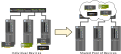
\includegraphics{pooling}
    \caption
    [Pooling internal devices increases flexibility and improves resource utilization and cluster performance]
    {If machines could pool their internal devices, it would be possible to avoid queuing work on dedicated machines with particular device configurations. Instead, each machine could dynamically compose the \gls{io} infrastructure needed to meet a workload's \gls{io} requirements, by borrowing devices from other machines and releasing them when they are no longer needed.}
    \label{fig:device-pool}
\end{figure}

Cluster computing applications often have high requirements to \gls{io} performance.
%
%For example, compute accelerators, such as \glspl{gpu} and \glspl{fpga}, are often used to increase the processing speed of computing tasks.
For example, many computing clusters rely on compute accelerators, such as \glspl{gpu} and \glspl{fpga}, to increase the processing speed.
%
In recent years, we have also seen a convergence of the high-performance computing, big~data, and machine~learning research fields.
%
This development has led to new demands to \gls{io} performance where fast access to high-volume storage devices is becoming a requirement for high-performance computing, while low latency networking and making use of compute accelerators have become cloud computing issues~\cite{Trivedi2011,Coates2013,Taherkordi2018}.
%
If \gls{io} resources~(devices) are scarcely distributed in the cluster, cluster machines with \gls{io} resources may become bottlenecks, for example when a workload requires heavy computation on \glspl{gpu} or fast access to storage.
%
Contrarily, over-provisioning machines with resources may lead to devices becoming underutilized if a workload's \gls{io} demands are more sporadic.
%
Distributed processing workloads may even require a heterogeneous cluster design, with widely different compositions of devices and memory resources for individual machines in the cluster.
%
Being able to share and partition devices between cluster machines at run-time leads to more efficient utilization, as individual machines may dynamically scale up or down \gls{io} resources based on current workload requirements (\cref{fig:device-pool}).



In order to meet the latency and throughput requirements of data-driven and compute-heavy workloads, there is a need for flexible, yet efficient, sharing of \gls{io} resources in a networked computing cluster.
%
This dissertation contributes to this goal by presenting a solution that enables distributing devices and sharing memory resources between machines interconnected with \gls{pcie}~\cite{spec:PCIe}.
%
By leveraging memory mapping functionality supported by the \gls{pcie} networking hardware, we make it possible to use resources residing in remote machines as if they were installed in the same machine.
%
Whether resources are local or remote is made transparent to application software, \gls{os}, and even device drivers, and remote resources can be used in a manner that is indistinguishable from using resources attached to the local \gls{pcie} bus.
%
Existing device drivers and application software may use remote resources without requiring any adaptations.
%
Not only does this make it easier to increase the overall resource utilization in the cluster, but it also becomes easier to design and implement distributed applications as software no longer needs to be written with accessing remote resources in mind,
but can instead be implemented as if all resources are local.
%
Using our solution, \gls{io} resources are no longer locked to individual machines, and memory and devices can be shared freely with other machines in the cluster.
%
Scaling out and using more hardware resources than there are available in a single machine becomes easier, and our solution improves both the performance of individual machines and the entire cluster as a whole.



\section{Background and motivation}\label{sec:motivation}
In cloud computing environments, dynamically scaling resources is often accomplished through virtualization. 
%
\Gls{vm} \glspl{hypervisor} may dynamically add virtual \gls{io} devices to \glspl{vminstance} on demand.
%
It is even possible to temporarily suspend computation to migrate \glspl{vm} to \glspl{hostmachine} with more hardware resources available, should the requirements of a \gls{vmguest} exceed the available local resources.
%
However, when the raw, bare-metal \gls{io} performance is required, for example in the case of \gls{gpu}-intensive machine~learning workloads, resource virtualization may not be a viable solution.
%
In this regard, it is possible to \lgls{passthrough}{``pass through''} physical \gls{io} devices to a \gls{vmguest} using an \gls{iommu}.
%
The \gls{iommu} facilitates direct access to hardware from the \gls{guest} without compromising the virtualized environment~\cite{whitepaper:Abramson2006,Muli2006}.
%
As such, \gls{passthrough} allows physical hardware to be used by a \gls{vmguest} with minimal software overhead.
%
However, as physical devices are tightly coupled with the \gls{host} they are installed in, this \gls{passthrough} technique suffers from a lack of flexibility.
%
Distributing \glspl{vm} across \glspl{host} in the network in a way that maximizes resource utilization and adapts dynamically to varying \gls{io} requirements, without sacrificing the bare-metal performance that pass-through provides, remains a challenge.



Another challenge is the networking technology itself. 
%
Despite having been a research topic for decades, moving data to remote computing units over a network remains a costly operation that introduces large performance overheads compared to using local resources.
%
As such, many \glspl{nic} support zero-copy of application memory from one system to another through \gls{rdma}~\cite{Huang2012}.
%
\Gls{rdma} is not only used in many distributed shared-memory cluster applications, but is also frequently used for implementing \gls{io} resource \gls{disaggregation} in software.
%
For example, \glspl{nvme} may be \gls{disaggregated} and shared with remote systems with very low latency.
This is the case for \gls{nvmeof}, where \gls{rdma} is used to provide direct access and avoid going through the block-layer of the \gls{os} on the server~\cite{Guz2018}.
%
Similarly, the result of a \gls{gpu} computation may be copied out of \gls{gpu} memory and onto the network directly using \gls{rdma}, without being copied to system memory first and going through the network stack~\cite{Venkatesh2014}.
%
However, while \gls{rdma} allows data to be transferred efficiently over the network, translation between the network protocol and the local \gls{io} bus is unavoidable. 
%
Compared to accessing a local device, this protocol translation incurs latency overheads that are not insignificant.
%
Moreover, as \gls{rdma} requires the use of specific programming models like \gls{mpi}~\cite{Jiang2004}, \gls{disaggregation} solutions based on \gls{rdma} are usually implemented either as application-specific \gls{middleware}, or as part of the application itself.
%
The sharing capabilities of \gls{rdma} solutions are, therefore, often limited to a single type of device.
Sharing several types of devices, for example both \glspl{gpu} and \glspl{nvme}, usually requires multiple \gls{disaggregation} implementations, and integrating them with each other may be a challenge.



\begin{figure}
    \centering
    \begin{subfigure}{\linewidth}
        \centering
        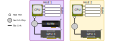
\includegraphics[width=.85\linewidth]{fabric-partitioning}
        \caption{Partitioning allows \glsfmtshortpl{cpu} and devices with different address domains to be isolated.}
    \end{subfigure}
    \par\vspace{5mm}
    \begin{subfigure}{\linewidth}
        \centering
        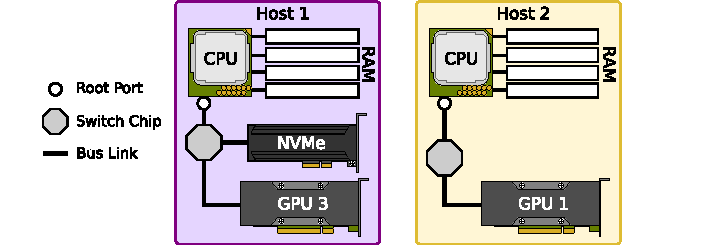
\includegraphics[width=.85\linewidth]{fabric-partitioning-device-tree}
        \caption{Machines have separate (logical) \glsfmtshort{pcie} device trees.}
    \end{subfigure}
    \caption[\Glsfmtshort{pcie} switch chips with partitioning support can be used to connect multiple \glsfmtshortpl{cpu} and freestanding devices to a common \glsfmtshort{pcie} fabric.]
    {\Glsxtrshort{pcie} switch chips with partitioning support can be used to connect multiple \glsxtrshortpl{cpu} and freestanding devices to a common \glsxtrshort{pcie} fabric. However, as systems are isolated, shared memory communication over \glsxtrshort{pcie} is not possible.}
  	\label{fig:partitioning}
\end{figure}



\begin{figure}
	\centering
    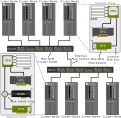
\includegraphics[width=.83\linewidth]{cluster-example}
    \caption[Example of a heterogeneous \glsfmtshort{pcie}-networked cluster with \glsfmtshort{ntb} adapter cards and external cables]{Example of a heterogeneous \glsxtrshort{pcie} cluster with external \glsxtrshort{pcie} links using adapter cards capable of \glsxtrshort{ntb}. The \glsxtrshortpl{cpu} as well as internal devices of all cluster machines~(nodes) are all attached to the same \glsxtrshort{pcie} network fabric.}
  	\label{fig:cluster-example}
\end{figure}



\begin{figure}
    \centering
    \begin{subfigure}{\linewidth}
        \centering
        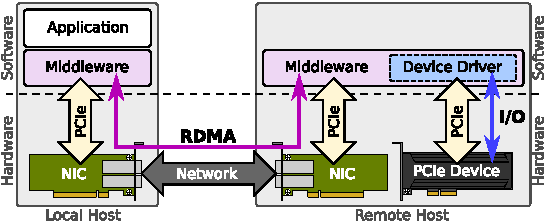
\includegraphics{direct-access-rdma}
        \caption{Accessing remote resources over traditional network using \glsxtrshort{rdma}.}
    \end{subfigure}
    \par\vspace{5mm}
    \begin{subfigure}{\linewidth}
        \centering
        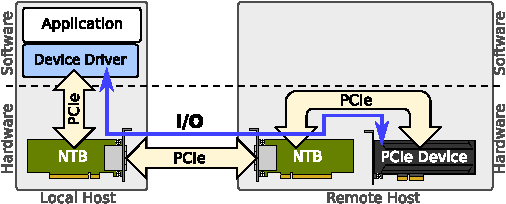
\includegraphics{direct-access-smartio}
        \caption{Accessing remote resources over native \glsxtrshort{pcie} using \glsxtrshort{ntb}.}
    \end{subfigure}
    \caption
    [Remote hardware can be accessed directly without any software in the critical path by using \glsfmtshortpl{ntb}]
    {Many distributed \gls{io} solutions have performance overheads because they rely on \gls{middleware} or other forms of software facilitation on the remote system. By setting up memory mappings through the \glsxtrshort{ntb}, remote hardware resources can be accessed directly without any software in the critical path.}
    \label{fig:direct-access}
\end{figure}



Extending the \gls{pcie} bus out of a single computer system and using it as a high-speed interconnection technology is a compelling alternative to distributed \gls{io} over a traditional network~\cite{whitepaper:Regula2004,Fountain2005,Ravindran2008}.
%
As \gls{pcie} is the standard for connecting \gls{io} devices to a local computer system, using only native \gls{pcie} would have clear performance advantage, since conversion between network protocol and \gls{io} bus would not be necessary.
%
However, since \gls{pcie} was originally designed to connect devices to the local \gls{cpu} on a motherboard, individual computer systems operate with different \gls{pcie} address domains.
%
Because of this, some \gls{pcie} switch chip hardware have virtualization support for dynamic partitioning~\cite{Chung2018,whitepaper:IDT,whitepaper:Microsemi}.
%
Multiple \glspl{cpu} can be connected to the same \gls{pcie} fabric by mapping partitions to the individual address domains of each \gls{cpu}.
%
Additionally, devices can be attached directly to the partitionable switch chip, rather than being owned by individual machines.
%
This allows switch-attached devices to be logically assigned to different machines, as illustrated in \cref{fig:partitioning}.



Nonetheless, because partitioning isolates \glspl{cpu} in separate address domains, this approach does not make it possible for machines to share their \emph{internal} resources.
%
Memory, or other devices that are attached to the local \gls{pcie} bus and not the partitionable switch (chip), cannot be shared.
%
Thus, partitioning lacks the shared-memory capabilities needed to support host-to-host communication over native \gls{pcie}, and other networking technologies, such as Ethernet or InfiniBand, must be used instead.
%
Consequently, \gls{disaggregating} devices and sharing them with multiple machines at the same time require either alternative methods, like \gls{rdma}, or additional virtualization support in the device itself,~i.e., \gls{sriov}.
%Distributed applications must instead use other networking technologies to communicate, such as Ethernet or InfiniBand, 
%
While approaches using \gls{pcie} fabric partitioning can be said to enable a composable \gls{io} infrastructure~\cite{Chung2018}, they stop short of providing \emph{networking} capabilities over \gls{pcie}.



Due to its intrinsic memory addressing abilities and low latency overhead, it is desirable to use \gls{pcie} as the enabling networking technology for distributed, shared-memory communication~\cite{Shim2018,url:Meduri2011}.
%
This requires translating memory transactions from one machine's address domain to another.
%
By far, the most common way of translating addresses between different \gls{pcie} address domains is by using a special type of device called a \gls{ntb}~\cite{whitepaper:PLX,whitepaper:Regula2004,Tu2014}.
%
%\Glspl{ntb} can be embedded as a \gls{cpu} feature~\cite{whitepaper:Sullivan2010,url:LinuxNTB-AMD}, but are more commonly implemented in \gls{pcie} switch chips~\cite{whitepaper:PLX,pex8733}.
%
%Using such \gls{ntb}-capable switch chips to implement peripheral devices and cluster switches, it becomes possible to connect independent computer systems with plug-in host adapter cards and external cables, as depicted in \cref{fig:cluster-example}.
By using \glspl{ntb} to implement plug-in host adapter cards and cluster switches, it becomes possible to connect independent computer systems as depicted in \cref{fig:cluster-example}.
%
The memory address translation capabilities of \glspl{ntb} make it possible for a machine to map (parts of) the address space of remote systems.
%
Since all memory address translations are done in the \gls{ntb} hardware, memory-to-memory transfers are supported with very low latency.



More interestingly, however, is the fact that in such \gls{ntb}-based networks, all \glspl{cpu} and internal \gls{pcie} devices are attached to the same, shared \gls{pcie} fabric.
%
Remote resources, such as the internal memory and devices of other machines, could be mapped into a local system and accessed through the \gls{ntb} with very little performance overhead.
%
Similarly, a device capable of \gls{dma} could also use the \gls{ntb} to access remote resources.
%
This approach eliminates the need to use memory on the remote system as an intermediate step when transferring data, and any software in the data transfer path can be avoided entirely, as shown in \cref{fig:direct-access}.
%
Rather than relying on dedicated servers or requiring that devices are attached to special switches, we could create distributed, peer-to-peer sharing system using \glspl{ntb};
%
\emph{all} machines in the cluster can share \emph{all} of their resources, including internal \gls{pcie} devices and system memory. 
%
Moreover, as centralized servers can be avoided, the risks of individual machines becoming performance bottlenecks or single points of failure are reduced.




However, using an \gls{ntb} to map remote resources requires awareness of the address space on the remote system.
%
For example, a device driver must use addresses that correspond to the remote device's address space when initiating \gls{dma} transfers.
%
Extensive modifications to device driver software would be required in order to manage multiple address space layouts.
%
This is infeasible due to the vast amount of devices and device driver implementations that exist. 
%
Although we could use virtualization to hide the fact that devices are on the other side of an \gls{ntb}~\cite{Tu2013}, by relying on \glspl{vm} we would forgo the possibility of using bare-metal machines for processing.
%
Hence, a realistic solution based on \glspl{ntb} requires a mechanism for abstracting away the physical location of a resource, as well as the address space of the machine it is installed in, without requiring virtualization (although sharing to \glspl{vm} should \emph{also} be supported).



Nevertheless, this kind of abstraction gives rise to yet another challenge.
%
A device driver that is unaware that a device is remote may assume that the entire local address space can be reached by the device.
%
\Gls{ntb} maps must be in place \emph{before} the driver interacts with the device, but predicting in advance which memory addresses a device driver may use is generally not possible.
%
Deferring the action of mapping through the \gls{ntb} until a time when addresses may be known is not realistic, as this would require synchronizing with the remote system and introduce communication overhead in the performance-critical path.
%
A way to prepare the necessary memory-maps through the \gls{ntb}, without adding communication latency, is needed.




\section{Problem statement}\label{sec:problem}
Utilizing \glspl{pcientb} to share resources among machines in a \gls{pcie}-networked cluster requires a solution for abstracting away the physical location of a resource, including the address space of the computer system it is installed in. 
%
More specifically, as it is desirable to avoid modifications to existing device drivers and application software, such a solution must also be able to present resources to the system as if they were locally installed.
%
Additionally, the solution must also allow remote resources to be used with the same performance expected for native \gls{pcie},~i.e., with the same performance as if they were attached to the local \gls{pcie} bus.
%
Hence, the goal of this dissertation is to develop a framework for sharing and distributing \gls{io}~resources (devices and memory) in a way that makes it indistinguishable if a resource is remote or local.
%
The challenges of this goal are addressed under the following research question: 
\begin{restatable}{question}{researchquestion}\label{question}
    Can \glspl{ntb} be leveraged to allow the internal memory and devices of individual computers in a \gls{pcie}-networked cluster to be shared with and used by remote machines in the cluster, as if these resources were local to the remote machines?
\end{restatable}
%
In particular, this research~question can be broken down into the following six objectives:


\begin{objective}\label{obj:distributed}
    Ubiquitous sharing in the cluster should be supported, allowing any machine to contribute any of its internal \gls{pcie} devices, and allowing any machine to be able to use shared devices, even contributing and using devices at the same time.
\end{objective}
The main motivation for our goal of building a system for \gls{io} resource sharing is to make it easier to scale out and use more resources than there are available in a single computer. 
If any standard \gls{pcie} device inside any machine could be shared with other machines, the \gls{io} resource utilization in the cluster could be greatly increased.
Additionally, by avoiding dedicated servers and allowing all computers in the cluster to participate in the sharing, contributing their own resources and using resources shared by others, we would effectively enable a distributed, peer-to-peer sharing model. 
This objective sets our goal apart from existing \gls{pcie}-based solutions, as these require a central server or devices that are directly attached to a \gls{pcie} switch.



\begin{objective}\label{obj:transparent}
    The fact that resources may be remote should be functionally transparent, allowing systems to use remote resources in the same way as if they were local, without requiring any modifications to device hardware, device drivers, host \gls{os}, or application software.
\end{objective}
If the solution could make remote devices behave as if they were locally installed, presenting resources to the system on a level ``underneath'' the \gls{os}, it would become possible to distribute devices to \emph{physical} hosts as well, and not only \glspl{vm}. 
In other words, remote resources should appear as if they were part of the local \gls{pcie} device tree, and application software could make use of remote devices using native interfaces in the same way it would use local devices.
%
Furthermore, by avoiding application- or device-specific \gls{middleware}, and instead memory-mapping remote system and device memory directly, existing device drivers and even the host \gls{os} itself would be able to interact with remote resources natively.
Avoiding any special adaptions to software would make scaling out significantly easier than what is currently possible with existing \gls{middleware}-based solutions for distributed \gls{io}, particularly those based on \gls{rdma}.



\begin{objective}\label{obj:performance}
    The fact that resources may be remote should be transparent with regard to performance, remote resources should be used with native \gls{pcie} performance, and as close to local access as possible.
\end{objective}
Moving data to remote units over the network introduces large performance overhead compared to accessing local resources. 
In order to further blur the hard separation between ``remote'' and ``local'', remote resources should not only behave functionally as if they were locally installed in the system using them, but also have comparable performance.
To achieve this, any communication overhead and intermediate data copying in the critical path must be completely avoided, a requirement that rules out (most) traditional methods of sharing resources over a network. 
Remote resources should be accessed directly over \emph{native} \gls{pcie}, which would improve the overall \gls{io} performance in the cluster.



\begin{objective}\label{obj:dynamic}
    Shared resources should be distributed \emph{dynamically}, and direct access to device memory and system memory should be configured at run-time, also between multiple devices residing in different hosts.
\end{objective}
As stated in \cref{obj:transparent}, the solution should work for physical hosts, and not only \glspl{vm}. Therefore, it must be possible to assign and reassign resources while all machines in the cluster are running, without requiring rebooting hosts or changing settings in the \gls{bios}.
For devices, this introduces the requirement that the \gls{os} supports \gls{hotadding} devices to the system (which most modern \gls{os} implementations do).
Not only would this would allow systems to dynamically scale up or down their \gls{io} resources based on immediate workload requirements, but devices could be more efficiently partitioned between machines in the cluster, increasing the overall resource utilization. 
Furthermore, the solution should also be able to automatically discover resource location, without requiring that the user knows anything about the underlying \gls{pcie} network topology, and dynamically set up memory mappings between devices, \glspl{cpu}, and memory resources. An example would be enabling \gls{pciep2p} between two or more \gls{dma}-capable devices that are physically installed in different machines.

    
\begin{objective}\label{obj:disaggregation}
    \Gls{disaggregation} of system memory, device memory, and device \emph{functionality} should be supported, and the solution should be able to distribute component parts to different hosts, as well as provide software facilities for resources that do not support \gls{disaggregation} in hardware.
\end{objective}
Because most device drivers are written in a way that assumes exclusive control over a device, some devices implement virtualization support in hardware,~i.e., \gls{sriov}, that makes them appear to a system as having multiple \glspl{vf}. 
%
The solution should be able to \gls{disaggregate} such \gls{sriov}-capable devices, and distribute their \glspl{vf} to different machines, allowing multiple computers to use the same device simultaneously.
%
However, since not all devices implement \gls{sriov}, the solution should also provide a device driver \gls{api} that will make it possible to \gls{disaggregate} memory and device resources in software.
%
In addition to the native sharing capabilities described in \cref{obj:distributed,obj:transparent,obj:performance,obj:dynamic}, this \gls{api} 
would provide facilities for memory-mapping device registers as well as mapping \gls{sharedsegment} for a \gls{dma}-capable device.
%
Effectively, this would bring shared-memory concepts to device driver implementations, allowing device operation and device resources to become part of the same global address space as distributed cluster applications.
%
This would allow multiple machines to simultaneously share the same, non-\gls{sriov} device, as well as making it possible to combine traditional \gls{io} with \gls{pcie} cluster capabilities such as zero-copy data transfer and \gls{multicasting}.
%
Moreover, the \gls{api} should be designed so that a driver implementation does not need to consider the system-local address space of the computer system where a device is installed, thus alleviating the complexity of programming device drivers for remote devices using \glspl{ntb}.



\begin{objective}\label{obj:experiments}
    To prove real-world deployment capabilities, the solution should be tested on realistic and relevant workloads and benchmarks.
\end{objective}
In order to confirm that \gls{io} resources can be distributed to, and shared with, remote machines, a comprehensive performance evaluation covering all components of the implementation is needed.
%
As the solution should provide \emph{native} \gls{pcie} performance (\cref{obj:performance}), all parts should be thoroughly tested with latency and throughput in mind, in order to reveal any potential performance bottlenecks.
Standardized test suites should be used as far as possible, to prove that application software really can be unmodified (\cref{obj:transparent}).
%
Moreover, to demonstrate the completeness of the solution, the evaluation should also include workloads relying on different \gls{pcie} network topologies and include several types of devices, such as \glspl{nvme}, \glspl{gpu}, and \glspl{nic}.
%
Finally, a prototype device driver using the device driver \gls{api} (\cref{obj:disaggregation}) should be developed and evaluated. 
%
This driver should demonstrate that it is possible to implement a distributed device driver, \gls{disaggregating} a non-\gls{sriov} device in software, and sharing it with multiple machines. 
%
The driver should also demonstrate how it can rely on memory \gls{disaggregation} and shared memory capabilities to implement data path optimizations.



\section{Scope and limitations}\label{sec:scope}
The research presented in this dissertation contributed to a collaborative project between academia and industry, with Dolphin Interconnect Solutions~(Dolphin) as the industry partner.\footnote{Funded by the Research Council of Norway under the ``Unified PCI Express for Distributed Component Virtualization'' project (RCN/NFR \#235530), with additional contributions from the ``LADIO: Live Action Data Input/Output'' project (EU H2020 \#731970).}
%
The goal of this project was to develop a new framework for sharing devices and memory resources among computer systems connected with \gls{pcie}.
%
The scope of this dissertation is the implementation and performance evaluation of the fundamental mechanisms that make this framework possible: \textbf{the discovery, addressing, access, and use of remote \gls{pcie}-attached resources}.
%
We aim to support this for three different levels of sharing:
\begin{enumerate}
    \item Dynamically distributing devices to remote machines.
    \item Dynamically distributing (physical) devices to \glspl{vm} running on remote machines.
    \item Enabling \gls{disaggregation} of devices and memory resources in software, allowing them to be shared simultaneously by software processes running on several machines.
\end{enumerate}



Exploring resource sharing possibilities using alternative networking technologies, such as InfiniBand, is outside the scope of our dissertation.
%
The desired objectives for the sharing framework, as stated in \cref{sec:problem}, necessitate the use of \glspl{pcientb}. %due to their shared-memory nature and performance requirements.
%
Dolphin's \gls{ntb} adapter cards and cluster switches make it possible to build heterogeneous computing clusters in various network topologies.
%
\Cref{fig:cluster-example} is an example of such a cluster.
%
Memory mappings between machines are configured using Dolphin's existing \gls{ntb} driver, and application software may use the \gls{sisci} programming \gls{api} to interact with this \gls{ntb} driver in order to dynamically set up and tear down these memory mappings and implement shared-memory communication.
%
In order to fit our work into this existing cluster networking foundation, we rely on Dolphin's \gls{ntb} hardware and have implemented our sharing framework as part of their driver stack.
%
This makes it possible to extend existing functionality, rather than developing an entirely new \gls{ntb} driver from scratch.
%
To enable software \gls{disaggregation}, for example, we can add device-oriented semantics and device driver support functions to the already existing \gls{sisciapi}. 
%, instead of requiring that cluster application software must convert and translate and between different \glspl{api}.
%
Even so, it should be pointed out that while our specific implementation is building on Dolphin \glspl{ntb}, the ideas and concepts of our work are general, and can in fact be implemented for \emph{any} \gls{ntb} hardware that has similar capabilities.



Using our framework, both \gls{host}~machines and \glspl{vm} should be able to use shared devices.
%
In order to accomplish this, resources must to be presented to the system at the \gls{os}-level so that interactions with a device can be intercepted. 
%
This intercepting mechanism involves manipulation of device driver interfaces and requires a detailed understanding of \gls{os} internals.
%
For this reason, our framework is implemented for Linux, as its source code is available as open source and may be studied.
%
For the same reason, we have also extended the \gls{kvm} in order to support sharing devices with \glspl{vmguest}.
%
Regardless, we do not limit our work to a specific Linux distribution, as it is possible to support several different versions of the Linux kernel.
%
It should also be noted that for \glspl{vm}, there are no limitations for which \gls{os} may run in the \gls{guest}.



As per \cref{obj:distributed}, sharing of any \gls{pcie} device should be supported, from \gls{pcie}~1.0 devices up to \gls{pcie}~4.0 devices.
%
Our evaluation includes a wide range of common (and commodity) devices, like \glspl{nvme}, Ethernet~\glspl{nic}, and \glspl{gpu}.
%
However, the framework should also not require any modifications to existing device driver implementations or device hardware~(\cref{obj:transparent}).
%
While \gls{ntb} clusters can be anywhere from 2 up to 60~machines, in many different network topologies, a limitation of the evaluation of our implementation is that it for the most part includes scenarios with cluster networks of only a few machines, since devices can only be used by one machine at the time.
%
Nevertheless, more advanced network topologies and larger clusters (of up to 60~machines) are used in a few experiments, as our framework supports \gls{disaggregating} devices in software, allowing devices to be used simultaneously by many machines.



Finally, it should be mentioned that several related research topics emerge from enabling the envisioned sharing framework this dissertation aims for.
%
Examples include finding algorithms for scheduling workloads on different machines in the cluster in order to optimize resource utilization, or choosing the appropriate trade-off between fairness and workload performance requirements when provisioning resources to machines.
%
The security implications of allowing remote machines to use and control internal system resources is also something that becomes relevant in the context of this sharing framework.
%
A ``finished product'' should attempt to address most of these topics, and ideally include tools and services for managing resources and orchestrating workloads on the cluster level.
%
However, we consider this to be outside the scope of this dissertation, and we only focus on the fundamental mechanisms that enable the low-level sharing functionality.



\section{Research methodology}\label{sec:methodology}
Choosing an appropriate research methodology for problems in computer~science is challenging.
%
Many methodologies come with their own set of considerations and potential pitfalls~\cite{McGrath1981}.
%
Finding a methodology is not made easier by the fact that computer~scientists themselves do not seem to agree on the age-old philosophical question of whether computer~science should be considered applied mathematics, engineering, or a science~\cite{Denning2005}.


According to Eden~\cite{Eden2007}, computer~science as a discipline can broadly be divided into three different research paradigms:
\begin{itemize}
    \item The rationalist paradigm, which defines computer~science as a branch of mathematics. 
        The paradigm seeks certain, a~priori knowledge of systems or processes through means of deductive reasoning.
    \item The technocratic paradigm, which defines computer~science as an engineering discipline.
        The paradigm seeks probable, a~posteriori knowledge about systems or processes through implementation (or prototyping) and empirical validation in the form of testing.
    \item The scientific paradigm, which defines computer~science as a natural (empirical) science.
        The paradigm seeks both a~priori and a~posteriori knowledge about systems or processes by combining formal deduction and scientific experimentation.
\end{itemize}
Note that the technocratic concept of a ``test'' differs from scientific experiments, in that the purpose of the former is to establish to which extent a set of requirements are met, whereas the latter is designed to corroborate or refute a hypothesis.
%%
If a test fails (to meet a requirement), the implementation must be revised. 
%
If an scientific experiment ``fails'', it is the theory (or understanding) that must be revised instead.


An almost identical classification of paradigms is given by the ACM Task Force on the Core of Computer Science~\cite{Comer1989}.\footnote{ACM use the names ``theory'', ``design'', and ``abstraction'' for these paradigms instead.}
%
They additionally note that the three paradigms are intrinsically intertwined, as computer~science is both deeply rooted in mathematics and has its own theory, experimental method, and engineering---in contrast to most physical sciences, where the engineering disciplines that apply their findings are considered separate disciplines.
%
The three paradigms are therefore equally fundamental to computer~science.



The subject matter of this dissertation touches on several sub-areas of computer~science, including computer and hardware architecture, distributed computing, \gls{os} fundamentals, and communication networks.
%
While all three paradigms can be applied to these sub-areas~\cite{Comer1989}, it is the technocratic paradigm which lends itself best to answering the overall problem~statement of this dissertation~(\cref{sec:problem}).
%
Neither the rationalist nor the scientific paradigm are particularly well-suited.
%
It is unrealistic to make a model through a~priori knowledge alone, due to the complexity of the many different hardware and software components of real-world computer systems.
%
Similarly, the process of gathering data with the goal of understanding the behavior of an indeterministic system, in order to create a statistical model and make predictions about it, seems equally unfit in this context.



As many \gls{disaggregation} solutions already exist, the motivation for this dissertation is not simply to make it easier for machines to share resources efficiently, but to do so by using a new approach altogether:
%
we attempt to unify traditional device \gls{io} with distributed, shared-memory computing by utilizing the inherent memory mapping capabilities of \glspl{ntb}.
%
It is desirable to realize this approach by \textbf{building a working prototype}, in order to explore potential opportunities and weaknesses along the way.
%
As such, we have followed the technocratic paradigm by iteratively designing, implementing, and testing our solution according to the objectives given in \cref{sec:problem}:
%
\begin{itemize}
    \item 
        One of the mechanisms developed makes remote resources appear and behave exactly as if they were part of the local \gls{pcie} tree.
        %
        In order to not require any special adaptions of existing hardware, device drivers, or application software, this mechanism is completely transparent.
        %
        This mechanism must is thoroughly tested using a wide range of functionality tests, for many different types of devices and device driver implementations.
        %
        As we make a point of using unmodified hardware and software, commodity devices and widely available software, such as standard benchmarking tools and well-known applications, is used in the validation of our solution.
        %
        We also include tests using a variety of different cluster network topologies and machine configurations, including \glspl{vm}, to provide a complete functionality evaluation.

    \item 
        A wide range of latency and throughput benchmarks is used to measure the performance of the critical \gls{io} data path.
        %
        Since the solution allows machines to use the internal devices and memory in other (remote) machines as if these resources were locally installed, it is possible to rely on comparison testing.
        %
        Tests looking at individual \gls{io} operations, such as reading/writing to an \gls{nvme} or copying memory out of \gls{gpu} memory, can first be performed using local resources (without our solution) to establish a performance baseline.
        %
        Then, the tests can repeated for remote resources using our solution, allowing us to compare the results and subsequently identify which component of the solution that needs to be improved.
        %
        %Note that the different iterations and gradual improvements of our solution can be seen in \crefrange{paper:nossdav}{paper:tocs}.

    \item 
        Our implementation process should also identify and explore new possibilities that are enabled by the solution.
        %
        The strength of our shared-memory approach is best highlighted by demonstrating capabilities that other resource sharing solutions lack.
        %
        For instance, as \gls{cuda} unified memory~\cite{url:unified-memory} and \gls{gpudirect}~\cite{url:GPUDirect,url:Rosetti2014} can be supported by our solution, even for \glspl{gpu} that reside in \emph{different machines}, we have performed experiments with direct memory-to-memory transfers across the cluster network.
        %
        Other possibilities, such as exploiting memory \gls{disaggregation} to implement memory locality optimizations or using \gls{pciemulticasting} to replicate data across several machines in a single operation, is also explored.
        %
        We investigate not only how different cluster network topologies affect the data path, but also prove the flexibility of our solution and demonstrate several of the sharing scenarios that are made possible.

    \item
        Realistic and \gls{io}-intensive computing tasks,~e.g., machine~learning and image processing workloads, are used to put the solution under heavy load.
        %
        By running real-world applications using several \gls{io} resources, any accumulated effects of any performance overhead caused by the implementation that are not visible on their own should be revealed.
        %
        Moreover, this kind of stress testing also proves that the solution is stable and gives reliable performance for repeated runs, and that it does not have any unintentional side-effects that affect systems over time.
        %
        Finally, showing that the solution works for a realistic workload has the additional purpose of proving that scaling real-world applications is possible.

\end{itemize}
%
For the sake of convenience, functionality testing and the overall validation process is implicit in the performance experiments presented in this dissertation.
%
However, it should be mentioned that while the presented experiments primarily use Intel~Xeon as the \gls{cpu} architecture, and \glspl{nvme}, Ethernet~\glspl{nic}, and Nvidia \glspl{gpu} were used for shared resources, additional \gls{cpu} architectures and devices were also used during the development and validation phases.
%
This includes \gls{cpu} architectures like AMD and ARM, and other devices like \glspl{fpga}, AMD \glspl{gpu}, sound cards, and \gls{pcie}-attached cameras.


\section{Contributions}
This dissertation contributes to the topic of resource sharing and distributed \gls{io} facilitation in cluster computing systems, and has been presented in five peer-reviewed venues: two conference workshop publications, one short-length demonstration paper, and two journal articles.
These publications are included as \crefrange{paper:nossdav}{paper:tocs} and contain the bulk of the implementation details, particularly \cref{paper:tocs}, which presents the entire solution as a whole.

We have developed a framework called \emph{SmartIO} for sharing resources and distributing devices in a heterogeneous, \gls{pcie}-networked cluster.
%
In particular, the main contributions of this dissertation are listed as follows:
\begin{itemize}
    \item Testing and evaluation of the \emph{\gls{dl}} method for \textbf{distributing \gls{pcie} devices to remote systems} (see \cref{paper:nossdav,paper:mmsys}): 
        %
        using \gls{dl}, any standard \gls{pcie} device, such as \glspl{nvme}, \glspl{gpu}, \glspl{nic}, and \glspl{fpga}, may be assigned to a remote system. 
        %
        The device appears to the remote system as if it has been dynamically \gls{hotadded} to the system, allowing existing device drivers to use the device without requiring any modifications to software.

    \item Implementation of a \textbf{new method for distributing devices to \glspl{vm}} running on any host machine in the cluster (see \cref{paper:srmpds,paper:cc}): 
        %
        we have developed an extension to the \gls{kvm} based on the \emph{\gls{mdev}} interface, enabling direct access to remote physical hardware devices for \glspl{vmguest} and setting up memory mappings for the devices. 
        %
        This \gls{mdev} implementation includes a method for dynamically discovering \gls{guest}-physical memory layout. Using this \gls{mdev} extension, local and remote devices can be \lgls{passthrough}{``passed through''} to \glspl{vm} and used with bare-metal performance.
	
    \item Improvement of the \gls{dl} and \gls{mdev} methods by implementing \textbf{support for multiple devices} and \textbf{supporting devices in different physical machines} (see \cref{paper:srmpds,paper:cc}):
        %
        a method for resolving device memory addresses and setting up memory mappings, in a way that is transparent to both the devices and the device drivers, is implemented. 
        %
        This enables direct data transfers between multiple devices without violating the principle of making devices appear local to the system(s) using them.

    \item Extension of the \gls{sisci} shared-memory \gls{api} with new, \textbf{device-oriented programming semantics and support functions for writing device drivers as shared-memory applications} (see \cref{paper:tocs}):
    %
    this \gls{apiext} makes it possible to \gls{disaggregate} devices and device memory in software, similarly to \gls{rdma} \gls{disaggregation} solutions.
    %
	Unlike \gls{rdma} solutions, however, remote resources can be memory-mapped directly into the virtual address space of a software process.
	%
        Through our \gls{apiext}, device driver implementations may take full advantage of \gls{pcie} shared memory capabilities, such as remote memory access and \gls{multicasting}, without requiring awareness of the underlying \gls{pcie} topology and the different address domains of remote systems.
	%
	This makes it easier to optimize data flow through the \gls{pcie} network, as software no longer needs to be written with accessing remote resources in mind, but can be implemented as if resources are local.

\item Development of a \textbf{new distributed \gls{nvme} device driver}\footnote{The prototype \gls{nvme} device driver is open source and can be found at \mbox{\url{https://github.com/enfiskutensykkel/ssd-gpu-dma}}~.
    It has also been adapted and used in other research projects: \mbox{\url{https://github.com/ZaidQureshi/gpudirect-nvme}}~\cite{Qureshi2022}.}
    using our device-oriented \gls{apiext} (see \cref{paper:tocs}):
        although the \gls{dl} and \gls{mdev} methods make it possible to use existing device drivers, most device drivers are written in a way that assumes exclusive control over the device. Therefore, a distributed device (\gls{function}) may only be used by a single user at the time.
    %
    To demonstrate software-enabled \gls{disaggregation}, we have implemented an \gls{nvme} driver as a \gls{userspace} \gls{sisci} application.
    %
    As a proof of concept, we show that a single \gls{nvme} device can be shared and operated by multiple cluster machines simultaneously, without requiring \gls{sriov}.
	This driver also demonstrates how multiple sharing aspects of SmartIO may be combined, 
        by \gls{disaggregating} remote \gls{gpu} memory and enabling memory access optimizations, supporting writing to and reading from storage directly to \gls{gpu} memory.
        %
        The \gls{nvme} driver may even run as a \gls{cuda} application on a remote \gls{gpu}, allowing \gls{gpu} threads to read and write to storage without involving the \gls{cpu}.

    \item A \textbf{comprehensive performance evaluation} covering all parts of SmartIO and the implementation of performance optimizations (see \cref{paper:mmsys,paper:cc,paper:tocs}):
        %
        with the goal of not incurring any performance overhead beyond that of native \gls{pcie}, the performance of using remote resources with SmartIO is comparable to that of local access (in terms of latency and throughput).
        %
        To prove that SmartIO is a viable and efficient solution for \gls{io} resource sharing also for realistic scenarios, two different image classification workloads relying on multiple \glspl{gpu} and \gls{nvme} storage have also been tested.
	
\end{itemize}
%
Finally, it should be noted that the research of this dissertation has had impact on real systems, as several components of SmartIO have already been incorporated into the product line of Dolphin Interconnect Solutions, and others are currently being adapted for real-world deployment.\footnote{{\url{https://www.dolphinics.com/solutions/pcie_smart_io.html}}}


\section{Outline}
This dissertation describes the design, implementation, and evaluation of the SmartIO framework for efficient sharing of resources between \gls{pcie}-networked computers.
%
The complete framework is described in detail in \cref{paper:tocs}, with the individual components and parts explained in \cref{paper:nossdav,paper:srmpds,paper:cc}.
%
These papers also show the evolution towards the finished solution, including the gradual performance improvements of the different iterations.
%
The rest of this dissertation is organized as follows:
%
\begin{description}
    \item[\cref{chapter:smartio}]
        gives a brief summary of SmartIO.
        %
        We describe the initial idea and challenges for SmartIO, and provide a high-level overview of the implementation and its considerations.
        %
        We also present an overview of related work focused on \gls{io} resource sharing in cluster networks.

    \item[\cref{chapter:conclusion}]
        summarizes our work and presents ideas for future work.

    \item[\cref{paper:nossdav}]
        describes the initial implementation of the \gls{dl} component of SmartIO.
        %
        We evaluate how performance is improved by using \gls{dl} to enable \gls{dma} transfers directly between a \gls{gpu} and remote memory, compared to using \gls{rdma} to achieve the same.

    \item[\cref{paper:mmsys}]
        is a demonstration of how the \gls{dl} component can be used for a realistic video stream processing workload implemented for \glspl{gpu}.
        We demonstrate how real-time processing requirements can be met by using \gls{dl} to scale up the number of available \glspl{gpu}.

    \item[\cref{paper:srmpds}]
        presents the \gls{mdev} component of SmartIO and how we improved the initial \gls{dl} implementation with support for multiple devices residing in different machines. 
        %
        We evaluate how performance is improved by enabling \gls{p2p} \gls{dma} transfers directly between devices instead of needing to bounce data transfers via system memory, and also identify performance issues with relying on the \gls{iommu}.

    \item[\cref{paper:cc}]
        is an extension of \cref{paper:srmpds} and provides an extended evaluation of both \gls{mdev} and \gls{dl}.
        %
        We show how different cluster network topologies affect \gls{dma} performance, for both \glspl{hostmachine} and \glspl{vmguest}.
        %
        Additionally, we also describe how we improved the original \gls{mdev} component with a mechanism for detecting \gls{guest}-physical memory layout.

    \item[\cref{paper:tocs}]
        presents the entire SmartIO solution as a whole, with the final iteration of the \gls{dl} and \gls{mdev} components.
        %
        We also introduce the \gls{sisciapiext} that makes it possible to \gls{disaggregate} devices and memory resources in software, and a proof-of-concept device driver implementation that uses this extension.
        %
        A thorough and complete performance evaluation of \emph{all} parts and components of SmartIO is provided, in order to prove that the final implementation does not cause \emph{any} performance overhead compared to native \gls{pcie}.
\end{description}

